\subsection{Brukermedvirkning og deltagende design}
\label{chp: medvirkning}

\subsubsection{Brukermedvirkning}
Uttrykket \emph{brukermedvirkning} er sammensatt av to aspekter, \emph{bruker} og \emph{medvirkning}. For å forstå hva brukermedvirkning egentlig er må vi forstå de to aspektene enkeltvis. Vi må anerkjenne at det finnes flere typer \emph{brukere}. Det kan være toppledelsen, som bruker systemets output i sine analyser og strategiske avgjørelser. Det kan være mellomledere som er ansvarlig for, og overvåker, avdelinger som bruker systemet. Til sist har vi de ansatte som bruker systemet i sitt daglige arbeid. Det er ofte naturlig at alle brukergruppene tar del i utviklingsprosessen i større eller mindre grad. Toppledelsen må kanskje godkjenne systemet, og kan ha meninger om hva slags rapporter det skal generere. Mellomledelsen og andre ansatte kan bidra med innsikt i dagens arbeidsrutiner, problemer og workarounds, samt kravspesifikasjoner, ønsker til design og testing. Vi må også forstå at \emph{medvirkning} ikke er det samme som involvering, selv om de to uttrykkene ofte blir brukt om hverandre. I Cavaye (1995) finner vi definisjonene av (bruker)medvirkning og involvering som henholdsvis \emph{"a set of operations and activities performed by users"} i løpet av utviklingsprosessen, og \emph{"subjective psycological state"} som påvirker brukernes forestillinger, og dermed systemets grad av suksess.

\noindent
Brukermedvirkning finner vi i mange former og på flere nivåer. Som vi ser i tabell \ref{Beskrivelse av brukermedvirkning} kan medvirkning beskrives ved hjelp av flere attributter. 

\begin{table}[H]
\caption{Beskrivelse av brukermedvikrning (hentet fra Cavaye (1995))}
%\centering
\begin{tabular}{c c}
\hline\hline
\textbf{Medvirkningsattributter} & \textbf{Mulige verdier} \\ [2ex]
\hline
& alle brukere \\[-1ex]
\raisebox{1.5ex}{Type} & representativt utvalg av brukere \\ [2ex]
\hline
& rådgivende \\ & signeringsansvar  \\
\raisebox{2ex}{Grad} & del av teamet \\ & fullt ansvar \\ [2ex]
\hline
& teknisk design \\
\raisebox{1.5ex}{Innhold} & sosialt og teknisk design \\ [2ex]
\hline
& prosjektdefinering  \\ & kravspesifikasjon  \\
\raisebox{2ex}{Område} & utvikling \\ & testing \\ [2ex]
\hline
& formell \\
\raisebox{1.5ex}{Formalitet} & uformell \\ [2ex]
\hline
& innspill ignorert \\
\raisebox{2ex}{Innflytelse} & bidrag tatt i betraktning  \\ & innspill tas seriøst \\
\hline
\end{tabular}
\label{Beskrivelse av brukermedvirkning}
\end{table}

\begin{itemize}
\item Type medvirkning beskriver andelen av brukere som faktisk blir inkudert. Det er ikke alltid det lar seg gjøre å inkludere alle brukere i praksis. Da er det viktig å etterstrebe å ha et representativt utvalg av disse med i prosessen.
\item Grad av medvirkning viser til at brukere har forskjellig grad av ansvar gjennon sin medvirkning.
\item Innholdet i medvirkningen refererer til det faktum at brukerne kan involveres i forskjellige aspekter av utviklingsprosessen. Det er vanlig at brukere involveres i aktiviteter som forbereder det tekniske designet av systemet, men de kan også involveres i det sosiale designet, det vil si de menneskelige og sosiale effektene systemet vil ha.
\item Området medvirkningen angår vil variere gjennom de forskjellige fasene av utviklingsprosessen. Medvirkning fra brukerne er mer vanlig i forbindelse med å sette rammer for prosjektet, kravsspesifikasjon og testing enn gjennom selve utviklingen og kodingen av systemet.
\item Medvirkningen kan være formell, ved bruk av formelle grupper og team, eller uformell, med tilfeldige diskusjoner og oppgaver.
\item Inflytelsen brukerene faktsik har kan variere, og innspill fra disse kan vektlegges i forskjellig grad av utviklerene, alt fra å bli totalt ignorert til å bli tatt svært seriøst. Dette betyr at det kan legges ned mye ressurser i å la brukerne får komme med innspill, men at virkningen av disse beror på i hvilken grad disse blir tatt hensyn til.
\end{itemize}

\noindent
I mange år ble det sett som en selvfølge at brukermedvirkning hadde en signinfikant positiv effekt på en eventuell suksess for et informsjonsystem. Empiriske studier kan imidlertid ikke bevise at det alltid er en slik sammenheng \cite{Cavaye95}. Dermed ser det ut til at brukermedvirkning hverken er tilstrekkelig eller ytterst nødvendig for å garantere suksess for et informasjonsystem. 
Det er flere grunner til dette, sett fra både designers/utviklers og brukerens side. For det første har forholdet mellom bruker og designer/utvikler stor innvirkning på effekten av medvirkningen. Forskjeller i bakgrunn, erfaring og perspektiver kan føre til konflikter som igjen preger effekten av medvirkningen på en negativ måte. For det andre spiller det ingen rolle i hvor stor grad brukerne medvirker i prosessen dersom deres innspill blir ignorert. For det tredje vil de ansattes motstand mot endring kunne resultere i ubrukte systemer, eller bevisst sabotasje av implementeringen og endringsprosessen. Som beskrevet i avsnitt \ref{chp: motstand}, vil motstand mot endring kunne reduseres ved god informasjon og involvering (til forskjell fra medvirkning) av de ansatte. Dette må ikke sees som en motsetning til Cavaye (1995)s påstand om at medvirkning ikke er en garanti for suksess. Dette fordi informasjon til og involvering av de ansatte ikke nødvendigvis behøver å inkludere medvirkning, og fordi selv med medvirkning og innspill fra de ansatte er en ikke garantert å redusere motstanden tilstrekkelig for å sikre en suksessfull implementering av det nye systemet. \cite{Cavaye95}

\subsubsection{Deltagende design}
\label{dd}
Deltagende design er én av mange teknikker for å oppnå brukermedvikning.
Interessen for denne teknikken blir stadig større, og sees på som en god måte å blant annet sikre gode innspill fra brukere (for blandt annet analyse av dagens situasjon), gjensidig læring og bedring av arbeidsrutiner.

\noindent
Vi kan dele utvikling av informasjonsystemer i tre aspekter: analyse, design og praksis. Det kan være vanskelig å kombinere alle tre samtidig, og tidligere ble det sett på som svært positivt om man greide å kombinere to av disse. Mogensen og Trigg (1992) ser i sin studie på muligheten for å kombinere alle tre aspektene samtidig (figur \ref{Challenge_PD}).

\begin{figure}[H]
\centering
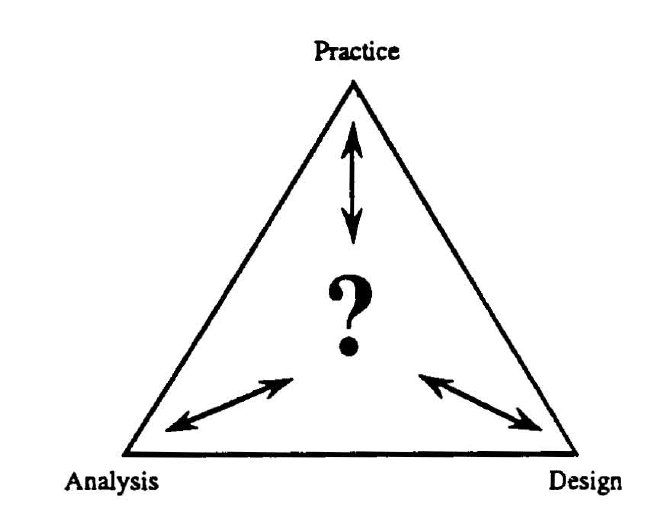
\includegraphics[scale=0.3]{Challenge_PD.jpg}
\caption{Hvordan kombinere alle?}
\label{Challenge_PD}
\end{figure}

\noindent
Ifølge \cite{Mogensen92} er det flere måter å oppnå større medvirkning på. Én teknikk er \emph{fremtidsworkshops}, der en ønsker diskusjon rundt mulige fremtidige løsninger på nåværende problemer, identifisert av brukerne selv. En annen teknikk er workshops hvor en bruker \emph{mock-ups og prototyper} for å trigge diskusjon om mulige fremtidige teknologier og løsninger. Uavhengig av valgt teknikk vil graden av relevans til dagens praksis være avgjørende for workshopens suksess. Felles for de to er at de tar i bruk kontekstuelle artefakter (artefakter medbrakt av fasilitator som brukerene selv setter i kontekst).

\noindent
Mogesen og Trigg (1992) konkluderer med at ved bruk av kontekstuelle artefakter kan lede til nettopp et slikt ønsket samspill (figur \ref{Artifacts_PD}). De argumenterer for at bruk av artefakter under en workshop ikke bare gir innspill på design - deltagende design, men at de også kan trigge diskusjoner som gir utviklerene bedre innsyn i dagens praksis, problemer og workarounds - deltagende analyse. 

\noindent
Deltagende design på denne måten, med bruk av kontekstuelle artefakter, gir derfor forskere/utviklere en dypere forståelse av hva som er problemområdene, og hvordan brukerne selv oppfatter dagens situasjon. Det gir også brukerne mulighet til større bevissthet rundt egne arbeidsmetoder, -rutiner og workarounds.

\begin{figure}[H]
\centering
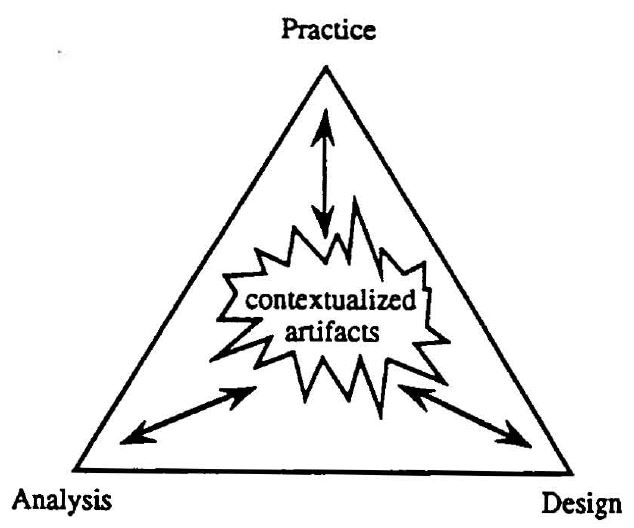
\includegraphics[scale=0.3]{Artifacts_PD.jpg}
\caption{Kontekstuelle artefakter støtter samspillet mellom de tre perspektivene}
\label{Artifacts_PD}
\end{figure}